\appendix
\chapter{Diagrammes du profile UML créé}

\section{Racine}
\begin{figure}[H]
    \begin{center}
    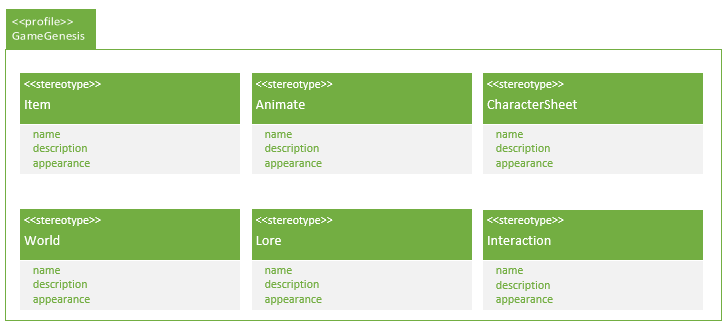
\includegraphics[width=14cm]{10_img/Z_annexeA/00.PNG} 
    \caption{Racine du modèle}
    \label{A-racine}
    \end{center}
\end{figure}

\newpage
\section{Item}
\begin{sidewaysfigure}
    \begin{center}
    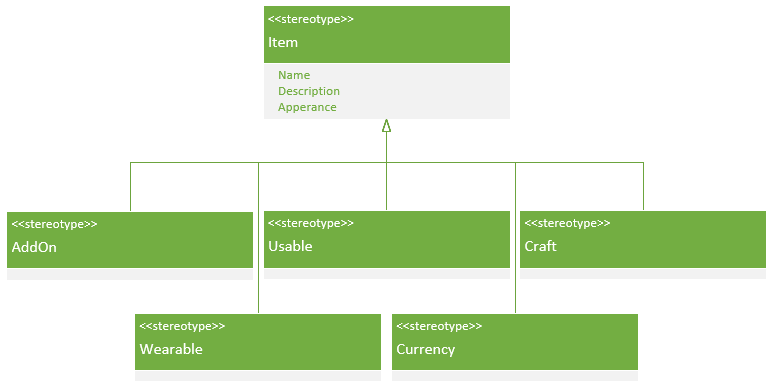
\includegraphics[width=20cm]{10_img/Z_annexeA/item_racine.PNG} 
    \caption{Item}
    \label{A-item-racine}
    \end{center}
\end{sidewaysfigure}

\newpage
\begin{sidewaysfigure}
    \begin{center}
    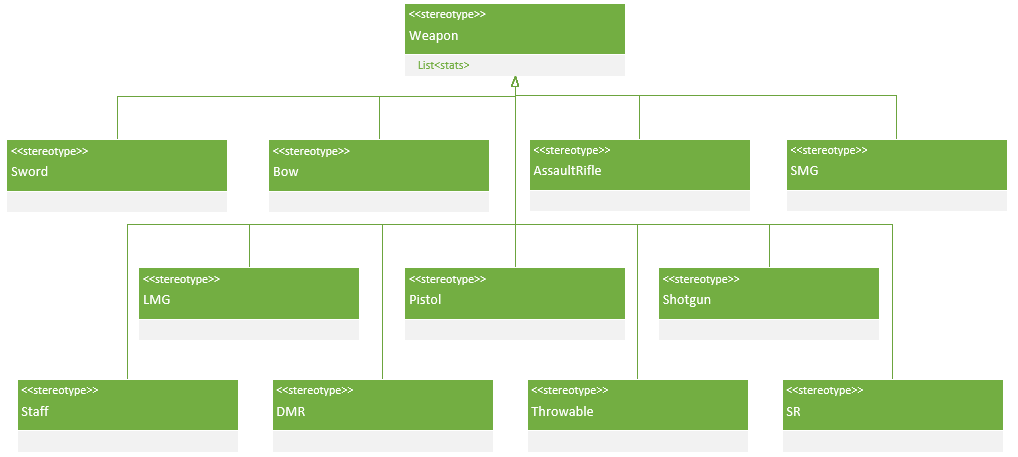
\includegraphics[width=20cm]{10_img/Z_annexeA/item_wearable_weapon.PNG} 
    \caption{Item - Wearable - Weapon}
    \label{A-Weapon}
    \end{center}
\end{sidewaysfigure}

\begin{sidewaysfigure}
    \begin{center}
    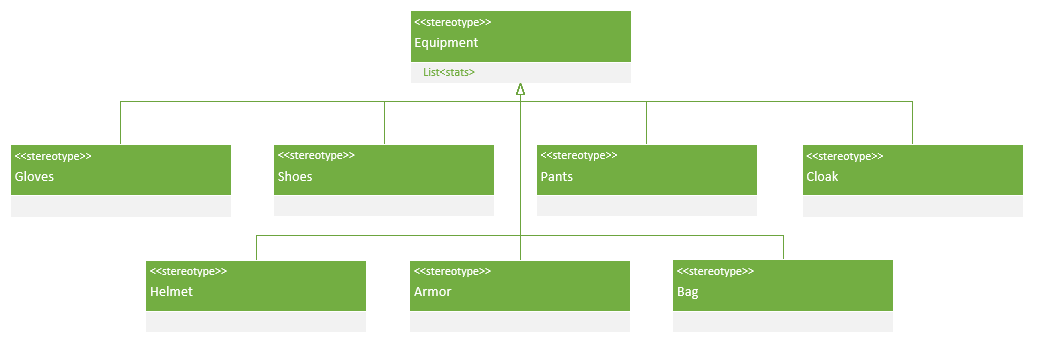
\includegraphics[width=20cm]{10_img/Z_annexeA/item_wearable_equipment.PNG} 
    \caption{Item - Wearable - Equipment}
    \label{A-Equipment}
    \end{center}
\end{sidewaysfigure}

\begin{figure}[H]
    \begin{center}
    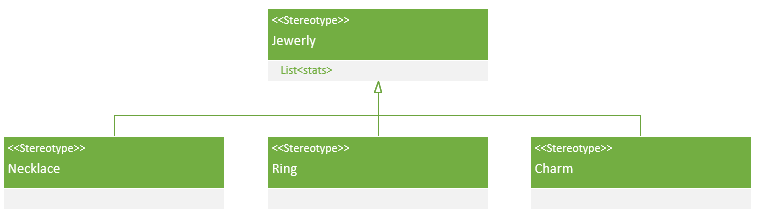
\includegraphics[width=14cm]{10_img/Z_annexeA/item_wearable_jewerly.PNG} 
    \caption{Item - Wearable - Jewerly}
    \label{A-Jewerly}
    \end{center}
\end{figure}

\begin{figure}[H]
    \begin{center}
    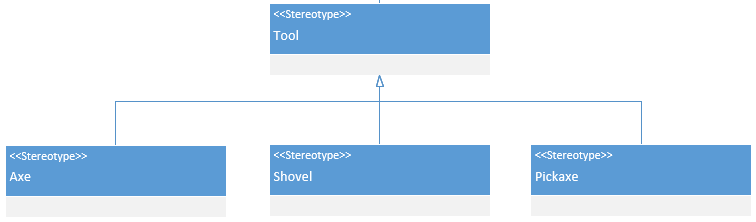
\includegraphics[width=14cm]{10_img/Z_annexeA/item_werable_tool.PNG} 
    \caption{Item - Wearable - Tool}
    \label{A-Tool}
    \end{center}
\end{figure}

\begin{figure}[H]
    \begin{center}
    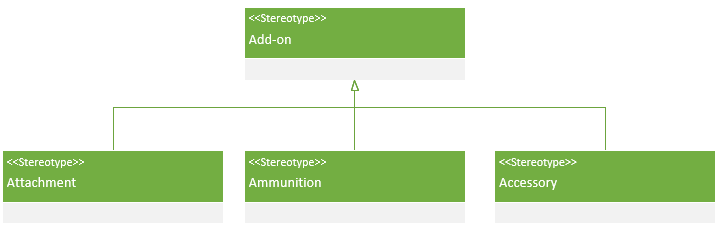
\includegraphics[width=14cm]{10_img/Z_annexeA/item_addon.PNG} 
    \caption{Item - Add-on}
    \label{A-Add-on}
    \end{center}
\end{figure}

\begin{figure}[H]
    \begin{center}
    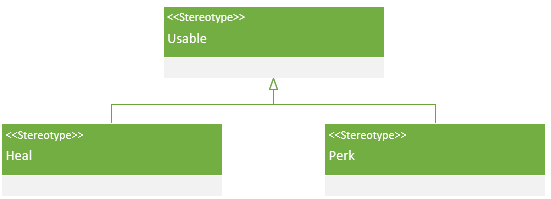
\includegraphics[width=10cm]{10_img/Z_annexeA/item_usable.PNG} 
    \caption{Item - Usable}
    \label{A-Usable}
    \end{center}
\end{figure}

\begin{figure}[H]
    \begin{center}
    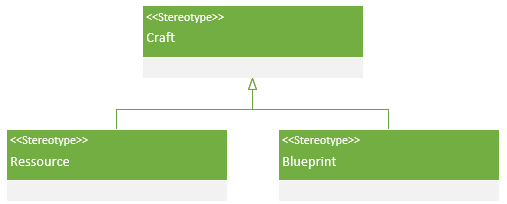
\includegraphics[width=10cm]{10_img/Z_annexeA/item_craft.PNG} 
    \caption{Item - Craft}
    \label{A-Craft}
    \end{center}
\end{figure}

\begin{figure}[H]
    \begin{center}
    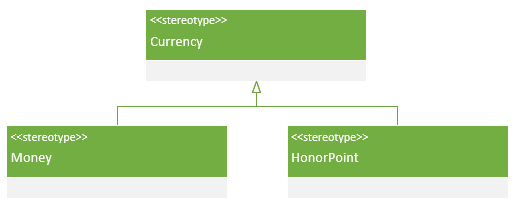
\includegraphics[width=10cm]{10_img/Z_annexeA/item_currency.PNG} 
    \caption{Item - Currency}
    \label{A-Currency}
    \end{center}
\end{figure}


\section{Animate}
\begin{sidewaysfigure}
    \begin{center}
    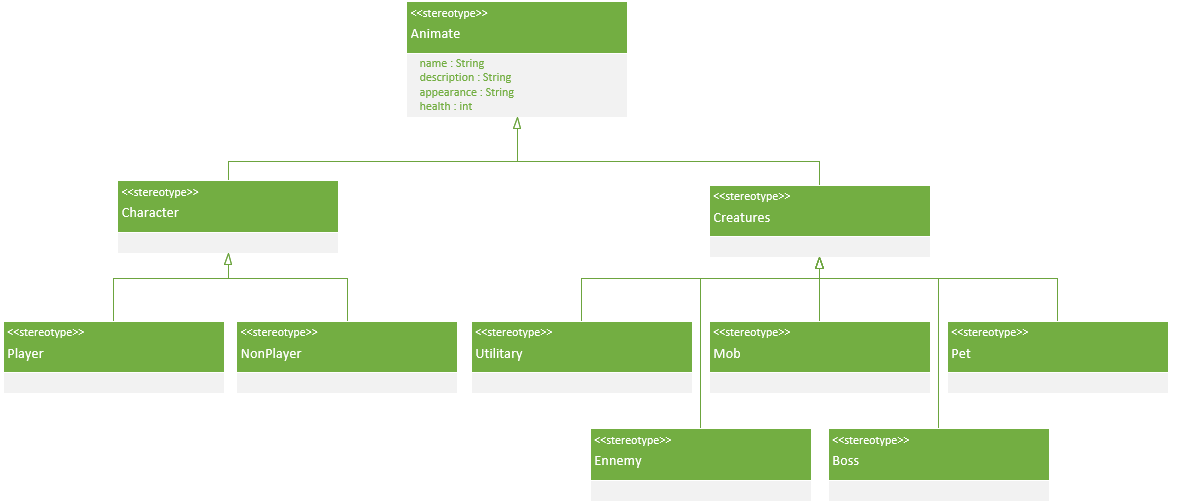
\includegraphics[width=20cm]{10_img/Z_annexeA/animate.PNG} 
    \caption{Animate}
    \label{A-Animate}
    \end{center}
\end{sidewaysfigure}



\section{Character Sheet} 
\begin{sidewaysfigure}
    \begin{center}
    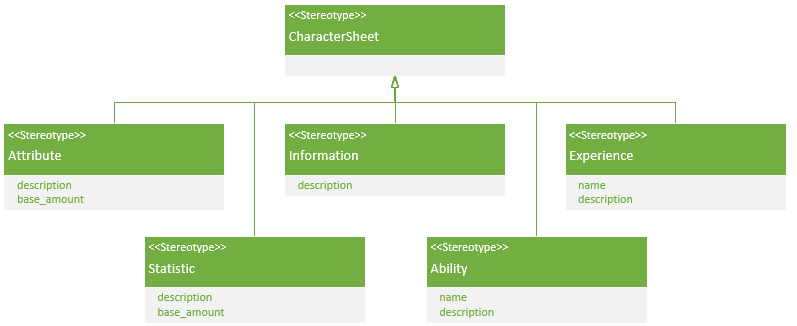
\includegraphics[width=20cm]{10_img/Z_annexeA/cs_racine.PNG} 
    \caption{CharacterSheet}
    \label{A-CS}
    \end{center}
\end{sidewaysfigure}

\begin{sidewaysfigure}
    \begin{center}
    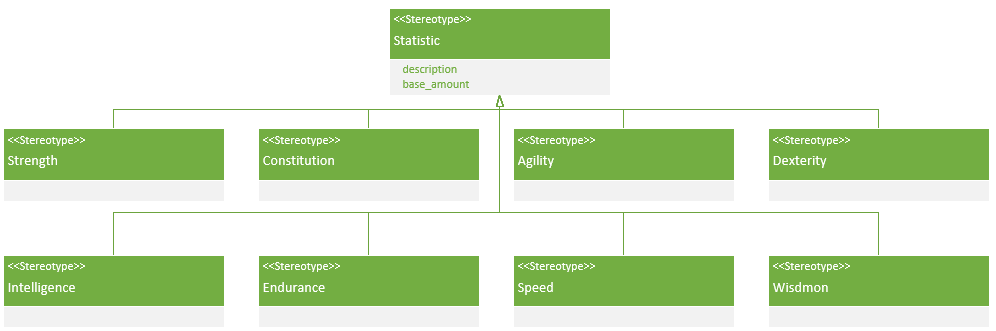
\includegraphics[width=20cm]{10_img/Z_annexeA/cs_statistic.PNG} 
    \caption{CharacterSheet - Statistic}
    \label{A-Statistic}
    \end{center}
\end{sidewaysfigure}


\begin{figure}[H]
    \begin{center}
    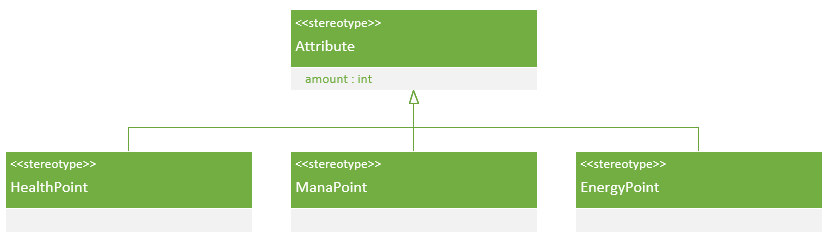
\includegraphics[width=14cm]{10_img/Z_annexeA/cs_attribute.PNG} 
    \caption{CharacterSheet - Attribute}
    \label{A-Attribute}
    \end{center}
\end{figure}

\begin{figure}[H]
    \begin{center}
    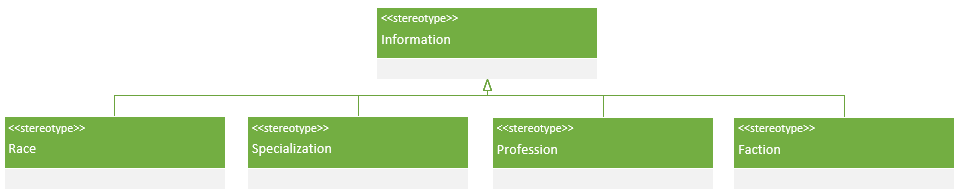
\includegraphics[width=15cm]{10_img/Z_annexeA/cs_information.PNG} 
    \caption{CharacterSheet - Information}
    \label{A-Information}
    \end{center}
\end{figure}


\section{LORE} 
\begin{figure}[H]
    \begin{center}
    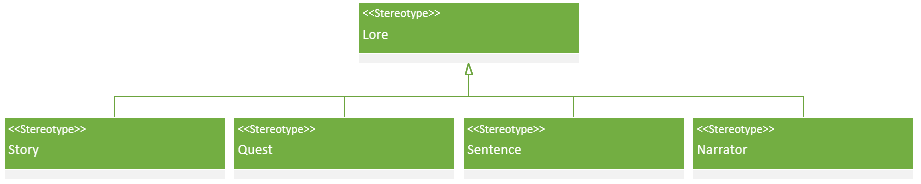
\includegraphics[width=15cm]{10_img/Z_annexeA/lore.PNG} 
    \caption{Lore}
    \label{A-Lore}
    \end{center}
\end{figure}


\section{World}
\begin{figure}[H]
    \begin{center}
    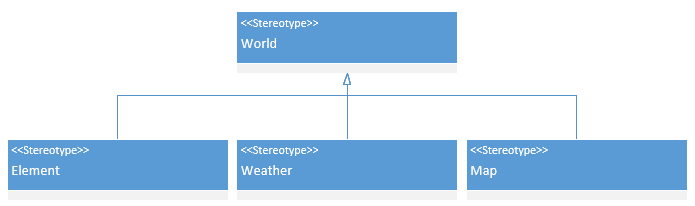
\includegraphics[width=14cm]{10_img/Z_annexeA/world.PNG} 
    \caption{World}
    \label{A-World}
    \end{center}
\end{figure}


\section{Interaction}
\begin{sidewaysfigure}
    \begin{center}
    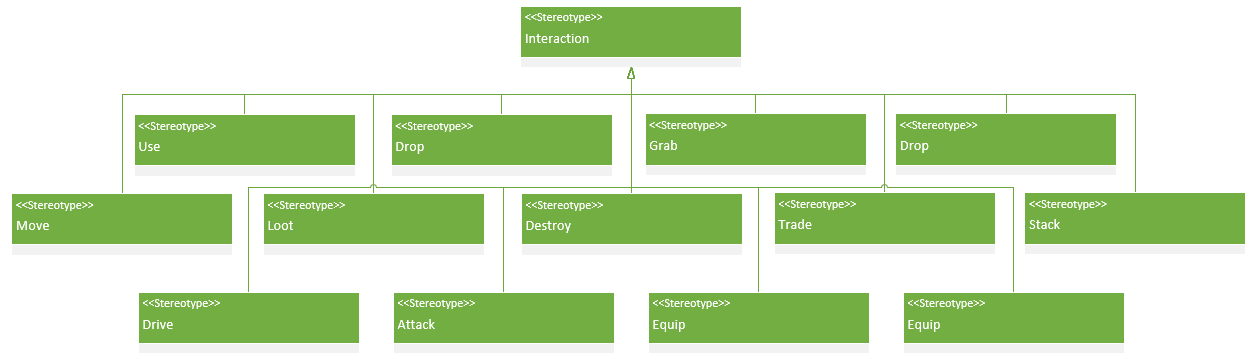
\includegraphics[width=20cm]{10_img/Z_annexeA/interaction.PNG} 
    \caption{Interaction}
    \label{A-Interaction}
    \end{center}
\end{sidewaysfigure}